\section{Réseaux de Petri}
Les Réseaux de Petri (abréviation  RdP) ont été introduits par le mathématicien Allemand Carl Adam Petri dans sa thèse \citep{Carl1962}, d'où leur appellation Réseaux de Petri (ou Petri Nets en anglais). Ces derniers méritent bien leur  appellation  car  la  thèse de C.A Petri a présenté un certain nombre d'idées fondamentales du modèle. Mais la théorie de RdP en sa totalité, telle que nous la connaissons actuellement est le résultat de fusionnement et de contribution directe ou indirecte des travaux de plusieurs  chercheurs de différentes universités et de différents laboratoires \citep{Robert2007}.

Les réseaux de Petri sont des outils à la fois graphiques et mathématiques permettant de modéliser le comportement dynamique des systèmes à  évènements discrets et d'évolutions simultanées. Leur représentation graphique permet de visualiser d'une manière naturelle le parallélisme, la synchronisation, le partage de ressources, les choix (conflits), etc. Leur représentation mathématique permet d'analyser le modèle pour étudier ses propriétés et de les comparer avec le comportement du système réel.

Ce section présente les notions fondamentales des réseaux de Petri.

\begin{definition}[Informelle]
Un réseau de Petri est un graphe biparti dont les sommets sont répartis selon deux types,  les places et les transitions. Ce graphe est constitué de telle sorte que les arcs du graphe ne peuvent relier que des places aux transitions ou des transitions aux places. Les places sont représentées par des cercles, alors que les transitions sont représentées par des traits ou des rectangles (Figure \ref{rdp}). Les places servent  à représenter les états du  système modélisé, tandis que les  transitions  représentent les changements d'état ou les événements \citep{SaidounicoursRdp2017}.

\begin{center}
	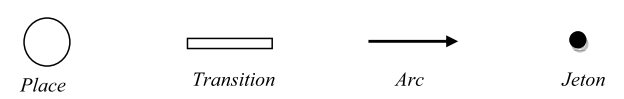
\includegraphics[scale=0.5]{img/rdp.PNG}
	\captionof{figure}{Représentation graphique des éléments de RdP} \label{rdp}
\end{center}


 Chaque place peut contenir un nombre entier de jetons. Les jetons modélisent souvent l'état d'une ressource (nombre d'instances, occupée ou non, ...). Un jeton est représenté par un petit cercle noir. Pour des commodités de présentation on met à l'intérieur d'une place le nombre de jetons présents (Figure \ref{place}). 
 
 \begin{center}
	
\includegraphics[scale=0.5]{img/place.PNG}
	\captionof{figure}{ Marquage d’une place } \label{place}
 \end{center}

 À  chaque arc est associé un nombre entier strictement positif appelé poids de l'arc. Lorsque le poids n'est pas signalé, il est égal à $"1"$  par défaut. Le RdP dont tous ses arcs sont de poids "1" est appelé RdP ordinaire (Figure \ref{rdpo}). Dans le cas o\`{u} les arcs peuvent avoir des poids supérieurs à $"1"$, il s'agit de RdP généralité (Figure \ref{rdpg}).
 
 \begin{center}
	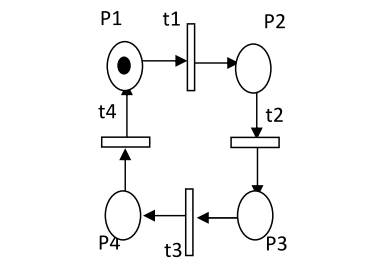
\includegraphics[scale=0.5]{img/rdp1.PNG}
	\captionof{figure}{RdP ordinaire} \label{rdpo}
 \end{center}
 
 \begin{center}
	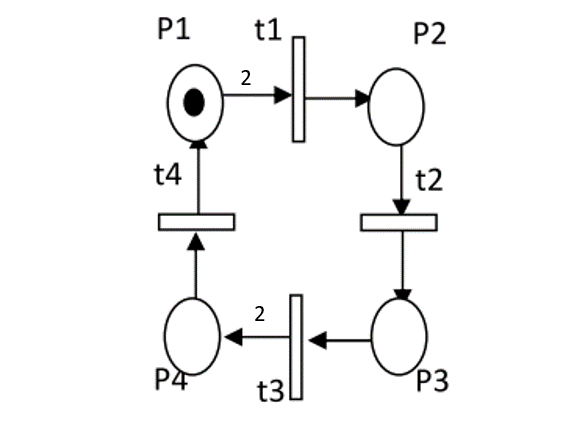
\includegraphics[scale=0.5]{img/rdpg.PNG}
	\captionof{figure}{RdP généralité} \label{rdpg}
 \end{center}
\end{definition}

\begin{definition}[Formelle]\citep{Murata1989}\\
Formellement un RDP est un quintuplet, $R= (P, T, Pre,Post , M_0 )$ tel que:
\begin{itemize}
	\item P : L'ensemble des places;
	\item T : L'ensemble des transitions;
	\item Pre : $(P  \times T)\rightarrow IN$, est l'application d'incidence avant, correspondant aux arcs directs reliant les
places aux transitions;
	\item Post : $(T  \times P)\rightarrow IN$,est l'application d'incidence arrière, correspondant aux arcs directs reliant
les transitions aux places;
	\item La matrice incidence du réseau est $C=Post-Pre$;
	\item $M_0$ : Le marquage initial (état initial). 
\end{itemize} 
\paragraph{Notation}
\begin{itemize}
	\item °t : L'ensemble des places d'entrée de la transition t;
	\item t° : L'ensemble des places de sortie  de la transition t;
	\item °p : L'ensemble des transitions  d'entrée de la place p; 
	\item P° : L'ensemble de transitions de sortie de la place p;  
\end{itemize}
Le RdP de la Figure \ref{rdp1} décrit le cycle des quatre saisons. Les places représentent les saisons,   $p_1$; le printemps, $p_2$; l'été,   $p_3$: l'automne et $p_4$: l'hiver. Les transitions représentent les changements de saisons, $t_1$; le début d'été, $t_2$; le début d'automne, $t_3$: le début d'hiver et $t_4$: le début du printemps. Le jeton dans la place $p_1$ indique que la saison à l'instant initial est le printemps. Ce scénario est modélisé comme suit:\\ 
$P= \{p 1 , p 2 , p 3 , p 4 \}$,\\ 
$T= \{t 1 , t 2 , t 3 , t 4 \}$, \\  
$Pre(p_1 ,t_1 )=1,\;\; 
Post(t_1 ,p_2 )=1,\;\; 
Pre(p_2 ,t_2 )=1,\;\; 
Post(t_2 ,p_3 )=1,\;\; 
Pre(p_3 ,t_3 )=1,\\ 
Post(t_3 ,p_4 )=1,\;\; 
Pre(p_4 ,t_4 )=1,\;\; 
Post(t_4 ,p_1 )=1$ ,  \\
$^{\circ}t_1=\{p_1 \},\;\; 
t_1^{\circ} =\{p_2 \},\;\; 
^{\circ}t_2=\{p_2 \},\;\; 
t_2^{\circ} =\{p_3 \},\;\; 
^{\circ}t_3=\{p_3 \},\;\; 
t_3^{\circ}=\{p_4 \},\;\; 
^{\circ}t_4=\{p_4 \},\;\; 
t_4^{\circ} =\{p_1 \}$,\\
$^{\circ}p_1= \{t_4 \},\;\; 
p_1^{\circ} = \{t_1 \},\;\; 
^{\circ}p_2= \{t_1 \},\;\; 
p_2^{\circ} =\{t_2 \},\;\; 
^{\circ}p_3= \{t_2 \},\;\; 
p_3^{\circ} = \{t_3 \},\;\; 
^{\circ}p_4= \{t_3 \},\;\; 
p_4^{\circ} = \{t_4 \}$.
 \begin{center}
	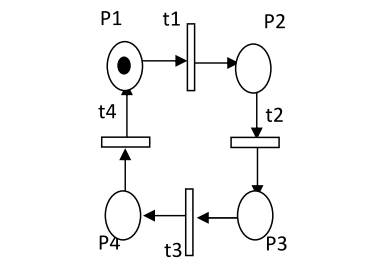
\includegraphics[scale=0.5]{img/rdp1.PNG}
	\captionof{figure}{Réseaux de Petri de quatre saisons} \label{rdp1}
 \end{center}
\end{definition}

\begin{definition}[Sensibilisation d'une transition]
Une transition $t$ est dite sensibilisée (validée, franchissable ou tirable) si chacune des places d'entrée $p$ contient un nombre de jetons supérieur ou égal au poids de l'arc reliant $p$ à $t$ \citep{SaidounicoursRdp2017}.  
$$ \forall p \in P, M(p) \geq  Pre (p, t) $$
\end{definition}

\begin{definition}[Franchissement d'une transition]
Le franchissement d'une transition $t$ sensibilisée retire de chacune de ses places d'entrée $p$ un nombre de jetons égal au poids de l'arc reliant $p$ à $t$ $(Pre (p, t))$ et dépose sur chacune de ses places de sortie p un nombre de jetons égal au poids de l'arc reliant $t$ à $p$ $(Post (p, t))$ \citep{SaidounicoursRdp2017}. Le franchissement d'une transition dans un marquage $M$ donne un nouveau marquage $M'$ défini par:
$$ \forall p \in P : M'(p)= M(p)+ C(p,t) $$

La Figure \ref{atom} illustre la réaction chimique $(2H_{2} + O_{2} \rightarrow 2H_{2}O)$ et le changement de marquage après le franchissement de la transition $t$. Avant le franchissement $M_ 0 =[2\; 2\; 0]$, après le franchissement $M_1 =[0\; 1\; 2]$. Les places sont ordonnées dans ce vecteur comme suit: $H_2 , O_2 , H_2 O$, le marquage de la place $H_2$ est noté par $M(H_2 )$. $M_0 (H_2 )$ est le marquage initial de la place $H_2$. Dans cet exemple $M_0 (H_2 ) =2$. 

\begin{center}
	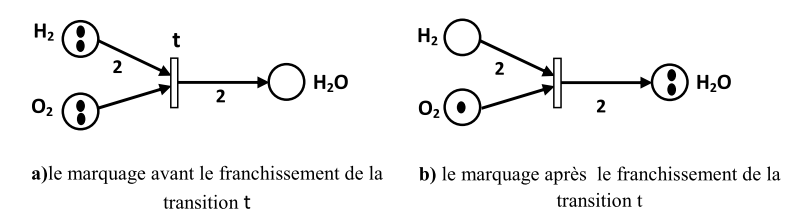
\includegraphics[scale=0.5]{img/H2O.PNG}
	\captionof{figure}{La composition d'eau $(2H_{2} + O_{2} \rightarrow 2H_{2}O)$ sous forme d'un RdP} \label{atom}
 \end{center}
\end{definition}\paragraph{Remarque }
 Lorsqu'une transition est validée, cela n'implique pas qu'elle sera immédiatement franchie; cela ne représente qu'une possibilité de franchissement, dans un  RdP, même si plusieurs transitions sont validées par un même marquage une et seulement une transition peut être franchie.
 
 
\begin{definition}[Graphe de Marquage]
Le graphe des marquages du réseau $G(R, M_0 $) est définit par un graphe orienté dont les sommets sont étiquetées par les marquages des états accessible $Acc(R, M_0 )$ et dont les arcs sont étiquetés par des transition de $L(R, M_0 )$.
Un marquage $M_i$  est accessible (atteignable) à partir de $M_0$ , s'il existe une séquence $s$ de franchissement des transitions qui permet d'atteindre $M_i$  à partir de $M_0$. On note: $M_0  [s > M_i  $


La construction du graphe de marquage $G$ est faite comme suit \citep{SaidounicoursRdp2017}:
\begin{itemize}
	\item Pour chaque marquage $M$ obtenu à partir de $M_0$, trouver toute les transitions franchissable $t_i$;
	\item Pour chaque transition $t_i$, trouver son marquage $M’$;
	\item Construire le nouveau nœud s'il est différent de celui déjà obtenu, puis ajouter l'arc correspondant au marquage actuel vers le prochain;
	\item Continuer l'exploration tant que des marquages et des transitions n'ont pas été encore considérés.
\end{itemize}
La Figure \ref{gm1} illustre le graphe de marquage obtenue à partir du RdP de la Figure Figure \ref{atom}.
\begin{center}
	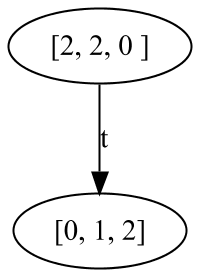
\includegraphics[scale=0.4]{img/gm1.PNG}
	\captionof{figure}{Graphe de marquage de $(2H_{2} + O_{2} \rightarrow 2H_{2}O)$} \label{gm1}
 \end{center}
\end{definition}

\begin{definition}[Système de transitions étiquetées]
Un système de transitions étiquetées appelé aussi $STE$ est un graphe orienté dont les sommets et les arcs de ce graphe orienté sont appelés respectivement états et transitions. Ces états et transitions sont associés avec une chaîne de caractères de manière à pouvoir les  distinguer entre eux.  Ces chaînes de caractères s'appellent \emph{noms} lorsqu'elles sont associées aux états, et étiquettes lorsqu'elles sont associées aux transitions .


Formellement un système de transitions étiquetées  est un quadruplet $\; STE = (S, Act, \delta, s_0)$ \citep{Saidouni2012}:
\begin{itemize}
	\item\textbf{S} est un ensemble (dénombrable) d'états;
	\item \textbf{Act}  est un ensemble (dénombrable) d'actions dites observables; 
 	\item  $\delta\subseteq \; S \times (Act \cup \{i\})$ : est l'ensemble des transitions, $i \notin Act$ est appelée action invisible (interne ou non-observable). Un élément $(x, a, y) \in \delta $ sera aussi noté par $x \stackrel{a}{\rightarrow}y$.
 	\item $s_0$ $\in\; S$ est l'état initial de $STE$. 
\end{itemize}

La Figure \ref{ste} illustre le STE du graphe de marquage de la Figure \ref{gm1}.
\begin{center}
	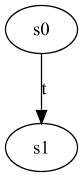
\includegraphics[scale=0.4]{img/ste.PNG}
	\captionof{figure}{STE de $(2H_{2} + O_{2} \rightarrow 2H_{2}O)$} \label{ste}
 \end{center}
\end{definition}

\begin{definition}[Structure de Kripke]
Une Structure de Kripke un graphe orienté dont les nœuds représentent les états accessibles du système et dont les arcs représentent les transitions entre les états. Une fonction d'étiquetage fait correspondre à chaque état un ensemble de propositions logiques vraies dans cet état \citep{Kripke1963}.

Formellement une structure de Kripke est un 4-uplet ${\displaystyle M=(S,I,R,L)}$ \citep{Edmund1999}:
\begin{itemize}
	\item \textbf{S} est un ensemble fini d'états;
	\item \textbf{I} $\subseteq$ \textbf{S} est un ensemble d'états initiaux;
	\item \textbf{R} $\subseteq$ \textbf{S}$\times$\textbf{S}  est une relation de transition qui vérifie: pour tout ${\displaystyle s\in S}$, il existe ${\displaystyle s'\in S} $ tel que ${\displaystyle (s,s')\in R}$;
	
Soit ${\displaystyle AP}$ un ensemble de propositions atomiques, c'est-à-dire des expressions booléennes portant sur des variables, des constantes et des prédicats. On note ${\displaystyle 2^{AP}} $ l'ensemble des parties de ${\displaystyle AP}$.
	\item \textbf{L: S} $\rightarrow 2^{AP}$ est une fonction d'étiquetage(ou d'interprétation) définit pour chaque état ${\displaystyle s\in S}$ l'ensemble ${\displaystyle L(s)}$ de toutes les propositions atomiques qui sont valides dans cet état.
\end{itemize}

\paragraph{Remarque}
La condition associée à la relation de transition ${\displaystyle R}$ spécifie que chaque état doit avoir un successeur dans ${\displaystyle R}$, ce qui implique que l'on peut toujours construire un chemin infini dans la structure de Kripke. Cette propriété est importante lorsque l'on traite des systèmes réactifs\citep{Klaus2004}. Pour modéliser un interblocage dans une structure de Kripke, il suffit de faire boucler l'état d'interblocage sur lui-même.


Un chemin dans la structure ${\displaystyle M}$ est une suite ${\displaystyle c=s_{1},s_{2},s_{3},\ldots }$ d'états tels que ${\displaystyle (s_{i},s_{i+1})\in R}$ pour tout ${\displaystyle i}$. L'étiquette du chemin est la suite d'ensembles ${\displaystyle w=L(s_{1}),L(s_{2}),L(s_{3}),\ldots }$,$\ldots$ qui peut être vu comme un mot infini sur l'alphabet ${\displaystyle 2^{AP}}$.

\end{definition}

La Figure \ref{stkrdp} représente une structure de Kripke dont l'ensemble de propositions atomiques est ${\displaystyle AP=\{p,q\}}$. Ici ${\displaystyle p}$   et ${\displaystyle q}$  sont des propriétés booléennes quelconques. L'état \emph{$s_1$} contient les deux propositions, les états \emph{$s_2$} et \emph{$s_3$} respectivement ${\displaystyle q}$  et ${\displaystyle p}$. L'automate admet le chemin ${\displaystyle c=s_1,s_2,s_1,s_2,s_3,s_3,s_3,\ldots }$, et le mot ${\displaystyle w=\{p,q\},q,\{p,q\},q,p,p,p,\ldots }$ est la suite des étiquettes associées.

\begin{center}
	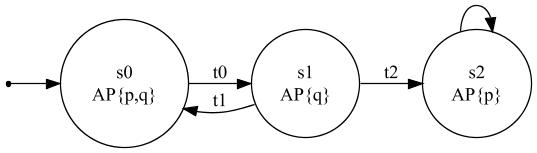
\includegraphics[scale=0.4]{img/stk.PNG}
	\captionof{figure}{Une structure de Kripke à trois états, avec deux propositions} \label{stkrdp}
 \end{center}
 
 
La distribution de l'espace d'états entrain la fragmentation de la structure de Kripke. Les structures partielles de Kripke modélisent des espaces d'états incomplets à parties inconnues (états border). L'évaluation des formules logiques temporelles sur les structures partielles de Kripke repose donc sur des interprétations à trois valeurs; la valeur de vérité supplémentaire \textbf{$\perp$ }  signifie « inconnu si la propriété est vraie ou fausse ».\\
Formellement une structure partiale de Kripke est un 4-uplet \\${\displaystyle F_M(T) = (S_T , I_T , R_T , L_T )}$ \citep{depriester2011bouneb}:
\begin{itemize}
	\item $T \subseteq S $;
	\item \textbf{$S_T$}  est une sous ensemble d'états fini de l'espace d'états S;
	\item \textbf{$R_T$} $\subseteq$ \textbf{$S_T$}$\times$\textbf{$S_T$}  est une relation de transition qui vérifie: pour tout ${\displaystyle s\in T}$, il existe ${\displaystyle s'\in S_T} $ tel que ${\displaystyle (s,s')\in R}$;
	\item $I_T$ est un ensemble fini d'états qui vérifie: pour tout $ s \in S_T $ tel que $ s \in I \}$;
	\item $ L_T$ : $S_T \times P \rightarrow \{ false, \perp , true \} $.
\end{itemize}

La Figure \ref{stkrdpd} représente des structures partielles de Kripke repartie sur trois machines, dont l'ensemble de propositions atomiques est ${\displaystyle AP=\{a,b,c\}}$. La répartition des états est fait comme suit:  
\begin{itemize}
 \item Sur la machine $M_1$ la structure partiale renferme deux  états à parties complets $s_0$ et $s_1$, et deux états à parties incomplets $s_2$ et $s_4$;
 \item Sur la machine $M_2$ la structure partiale renferme un état à partie complet $s_4$, et un état à partie incomplet $s_5$;
 \item Sur la machine $M_3$ la structure partiale renferme deux  états à parties complets $s_2$ et $s_5$, et deux états à parties incomplets $s_1$ et $s_4$
 \end{itemize}

\begin{center}
	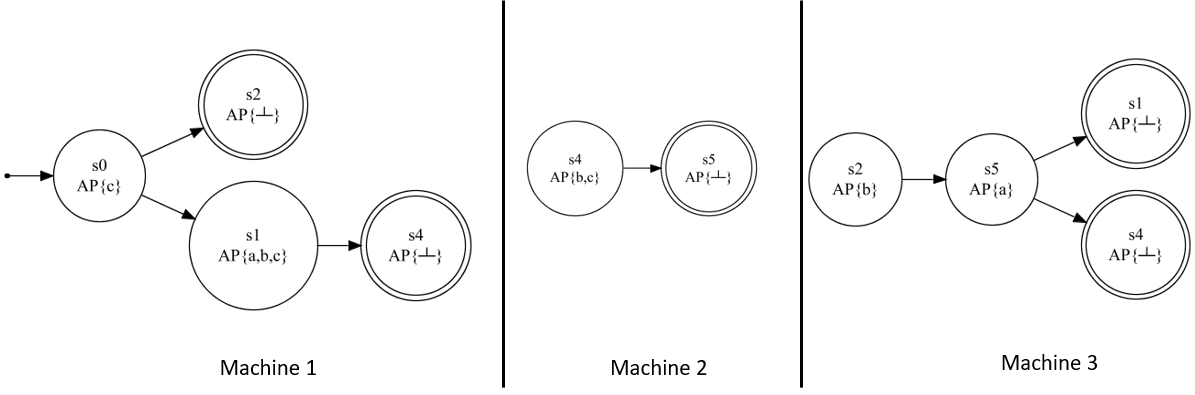
\includegraphics[scale=0.5]{img/stkd.PNG}
	\captionof{figure}{Une structure de Kripke à trois états, avec deux propositions} \label{stkrdpd}
 \end{center}